%The motivation of \gls{rp} usage to project 1D signal into a \gls{2D} space by embedding procedures is to identify time recurrences (correlations) that are not easily apparent in the \gls{1D} signals. These recurrences encode physiological states that can be assessed by searching repeated patterns in the produced 2D images. Similarly, \gls{mtf} can be employed to produce such representation, but by using a Markov chain of first order. Finally, the same end can be achieved using \gls{gaf}, which represents a time series in a polar coordinate system and then it builds a Gramian matrix where each element is the trigonometric sum between different time intervals. In the Gramian matrix, each element is, actually, the cosine of the summation of angles. These algorithms are suitable for characterizing signal quality because the images generated from them produce texture patterns highly correlated with the original waveform of the 1D signal. From Figure~\ref{fig:signals_and_maps}, we can notice that a noisy signal, customarily associated with ‘unreliable’ \gls{SQI}, often presents visual patterns with lower redundancies and higher entropy. On the other hand, reliable signals usually produce projections (or `encoding maps') with lower entropy and harmonious texture patterns.

%% OBSERVATION
%% Podemos omitir para o WCOMP, mas pode detalhar ainda mais na sua dissertação!
%\subsection{Gramian Angular Field}

% The main idea behind \acrfull{gaf} projection method is utilizing the polar coordinate system $ [0,\pi] \times \mathbb{R} $, to represent the signal in a way that the overall shape of the signal curve changes as time passes, since the arc of the circumference increases as the radius increases. Therefore, not mattering if the signal is periodical, its shape changes as time passes. 

% To map a linear signal to such a coordinate system, the following identities were applied to obtain the radius $r_i$ and the angle $\phi_i$ of the $i$-th sample of the signal: ${\phi_i = arccos(x_i)}$, with ${x_i \in \mathbb{R}}, {-1 \leq x_i \leq +1}$; and ${r_i = t_i/N, t_i \in \mathbb{N}}$, with ${N \in \mathbb{R}}$, where $N$ can be used to stretch or to detract the signal along the radius axis. Notice that the signal needs to be rescaled to the interval $[-1,+1]$. 

% However, the signal is yet one-dimensional. Hence, an aggregate operation $Agg$ is applied to each pair to produce the matrix $ GAF = \{Agg(\phi_i,\phi_j)\}_{i,j}$. Examples of those aggregate functions are the $cos(\phi_i + \phi_j)$ function, which produces the Gramian Summation Angular Field ($GAF_S$), and the function $sin(\phi_i - \phi_j)$, that produces the Gramian Difference Angular Field ($GAF_D$). They can be simplified by the use of trigonometric properties, as seen in the following equations:
% \begin{align}
%     GAF_S & = (\vec{x}^T \cdot \vec{x}) - ((\Delta(\vec{x}))^T \cdot \Delta(\vec{x})) = 
%     \cos^{-1}\left( \frac{T_{ij}}{\sqrt{T_{ii} \cdot T_{jj}}} \right) \\
%     GAF_D & = ((\Delta(\vec{x}))^T \cdot \vec{x}) - (\vec{x}^T \cdot \Delta(\vec{x})) = 
%     \sin^{-1}\left( \frac{T_{ij}}{\sqrt{T_{ii} \cdot T_{jj}}} \right)
% \end{align}
% Where $\Delta(\vec{v})$ applies the function $f(x)=\sqrt{1-x^2}$ to $\vec{v}$ element-wise. 

% \subsection{Markov Transition Field}

% The Markov Transition Field's first step is elaborating a Markov chain of first order, considering as states quantile bins containing samples of the signal and defining as a transition of states $S_i \rightarrow S_j$ as the probability of, given the set of all pairs $(x_u,x_{u+1})$ of subsequent signal samples for all $x_u \in q_i$, the subsequent sample $x_{u+i}$ belong to the quantile $q_j$. Then, the Markov chain can be described as the matrix ${M = \{P(S^\prime \rightarrow S_j|S^\prime=S_i)\}_{i,j}}$, where $S^\prime$ is the current state of the Markov chain state machine. Notice that $\sum_j P(S^\prime \rightarrow S_j|S^\prime=S_i) = 1$ for each state $S_i$.

% Nonetheless, the matrix $M$ doesn't fully retain the time sequentiality, since quantiles are sets obtained by value, not by timestamp. For that reason, a second step is made, building a matrix corresponding to the Markov Transition Field, defined as follows:
% \begin{equation}
%     MTF = \{M_{u,v} | x_i \in q_u, x_j \in q_v\}_{i,j}
% \end{equation}
% Where $M_{u,v}$ is the element of the matrix M on the given row and column.

% \subsection{Recurrence Plot}

% Finally, the last method is described, beginning with the transformation of the original signal $\vec{x}_{1 \times n}$ into a matrix $X_{d \times m}$, with $m=n-(d-1)$, where each of the $m$ columns corresponds to a vector $\vec{v}_j$ of $d$ dimensions, such that $\vec{v}_j=[x_j,x_{j+\tau},...,x_{j+\tau \cdot (d-1)}]$, that is, $\vec{v}_j$ is a sequence of $d$ samples of $\vec{x}$, beginning in the position $j$, with time delays of value $\tau$ between them. From that point of view, the matrix $X_{d \times m}$ can be seen as a vector $\vec{X}_m$ with elements of $d$ dimension.

% In the end, each distance between vectors contained in $\vec{X}$ can be compared, leading to the following matrix:
% \begin{equation}
%     RP = \{ D(\vec{X}_i, \vec{X}_j)  \}_{i,j}
% \end{equation}
% Where $D(\vec{X}_i, \vec{X}_j) = || \vec{X}_i - \vec{X}_j ||$. Optionally, it's possible to apply a threshold function $\Theta$ to classify the obtained distances, resulting in the matrix $RP = \{ \Theta(D(\vec{X}_i, \vec{X}_j))  \}_{i,j}$.

\section{Photopletysmograph signal}



\section{Projection Methods}

This section provides an analysis of the projections methods that this thesis used to convert the one-dimensional \gls{PPG} signal into a 2D representation. 

\subsection{Recurrence Plot}

% Introduzir aplicações e uso pretendido

The \gls{RP}, in essence, represents recurrences between the phase space values of time instant pairs. For this end, the first step is to embed the time series $X=x_1,x_2,...,x_n$ with $n$ samples into a phase space, creating a phase space series $S=s_1,s_2,...,s_m$ with $m$ elements. We can employ the time delays method to represent each element $s_i$ of this phase space $S$ as follows:

\begin{equation}
	s_i=\vec{s_i} = (x_i, x_{i + \tau}, x_{i + 2\cdot \tau} ..., x_{i + (d-1) \cdot \tau})
\end{equation}   

\noindent where $d$ is the dimension and $\tau$ is the time delay of the phase space. Notice that the lenght $m$ of the sequence $S$ depends on both $d$ and $\tau$ by the equation $m = n - (d-1) \cdot \tau$. 

Then, the second step is to build a $m \times m$ matrix $M$ of recurrences where each cell $M_{i,j}$ represents the presence or the ausence of a recurrence in a pair of points $\vec{s_i},\vec{s_j}$ of the phase space $S$. We can represent this concept by measuring the distance $||\vec{s_i} - \vec{s_j}||$ between the points of the pair and verifying if it is smaller than a threshold $\varepsilon$ as the following equation:

\begin{equation}
	M_{i,j} = \mathcal{H}(\varepsilon - ||\vec{s_i} - \vec{s_j}||)
\end{equation}

\noindent where $\mathcal{H}$ is the Heaviside function.  

% E se não tiver limiar?


\begin{figure}
	\centering
	\adjustbox{height=0.3\textheight}{
		\begin{tabular}{c}
			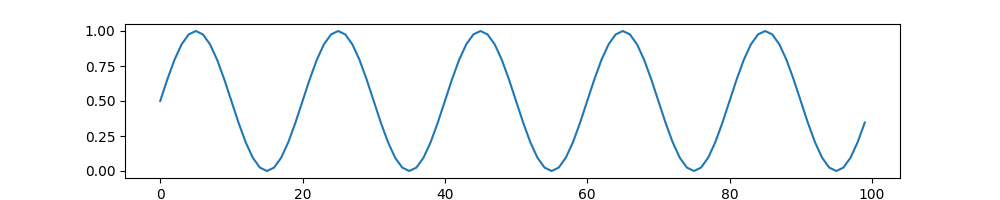
\includegraphics{img/middle_steps/signal.png} \\
			\includegraphics{img/middle_steps/delay_phase_space.pdf} \\
		\end{tabular}
	}
	\caption{}
\end{figure}

\subsection{Gramian Angular Field}

% falar sobre GAF

The \gls{GAF}, in summary, encodes the signal into angular relationships between pair of points. The first step to do this is to convert the signal $X=x_1,x_2,...,x_n$, with $n$ samples, into a polar coordinate series $P=p_1,p_2,...,p_n$. One manner to do that is to associate the time $t_i$ to the radius $r_i$ and the value $x_i$ to the angle by the inverse of the cosine as follows:

\begin{equation}
	p_i = (r_i, \phi_i),	
	\begin{cases} 
		\phi_i = cos^{-1}(x_i), & -1 \leq x_i \leq 1\\
		r_i = \frac{t_i}{N}, 	& t_i \in \mathbb{N}, N \in \mathbb{R}
	\end{cases}
\end{equation}    

The second step is to 

\begin{align}
	M_{i,j} & = cos(\phi_i + \phi_j) \\
		& = cos(\phi_i) \cdot cos(\phi_j) - sin(\phi_i) \cdot sin(\phi_j) \\
		& = x_i \cdot x_j - \sqrt{1 - x_i^2} \cdot \sqrt{1 - x_j^2}
\end{align}

\begin{equation}
	M = X^T \cdot X - \sqrt[\circ 2]{\mathds{1}-X^{\circ 2}}^T \cdot \sqrt[\circ 2]{\mathds{1}-X^{\circ 2}}
\end{equation}


\begin{align}
	M_{i,j} & = sin(\phi_i - \phi_j) \\
		& = sin(\phi_i) \cdot cos{\phi_j} - cos(\phi_i) \cdot sin(\phi_j) \\
		& = \sqrt{1 - x_i^2} \cdot x_j - x_i \cdot \sqrt{1 - x_j^2} 
\end{align}

\begin{equation}
	M = \sqrt[\circ 2]{\mathds{1} - X^{\circ 2}}^T \cdot X - X^T \cdot \sqrt[\circ 2]{\mathds{1} - X^{\circ 2}}
\end{equation}

\subsection{Markov Transition Field}

\begin{equation}
	W_{i,j} = \frac{\sum\limits_{x_k \in Q_i} \begin{cases} 
			0, & x_{k+1} \not\in Q_j \\
			1, & x_{k+1} \in Q_j
		\end{cases}}{|Q_i|}
\end{equation}


\begin{equation}
	M_{i,j} = W_{u,v} | x_i \in Q_u, x_j \in Q_j 
\end{equation}

